%%%%%%%%%%%%%%%%%%%%%%%%%%%%%%%%%%%%%%%%%%%%%%%%%%%%%%%%%%%%%%%%%%%%%%
%%%%%%%%%%%%%%%%%%%%%%%%%%%%%%%%%%%%%%%%%%%%%%%%%%%%%%%%%%%%%%%%%%%%%%
\documentclass[dvips,portrait]{cernsem}             %%%%%%%%%%%%%%%%%%
                                                    %%%%%%%%%%%%%%%%%%
%%%%%%%%%%%%%%%%%%%%%%%%%%%%%%%%%%%%%%%%%%%%%%%%%%%%
% gmake afb-LepEWG-ps
%======================



% The epsfig.sty is necessary to manage figures in postscript!
\usepackage{epsfig}

%%%=================local=macros=========================
\def\Order#1{${\cal O}(#1)$}
\def\OrderLL#1{${\cal O}(#1)_{\rm LL}$}
\def\Ordex#1{${\cal O}(#1)_{exp}$}
\def\Oceex#1{${\cal O}(#1)_{_{\rm CEEX}}$}
%
%
\def\Angle{$\theta^{\bullet}$}
%%%%\def\Angle{$\theta_1$}
\def\KK{${\cal KK}$}
%%%======================================================

%%%%%%%%%%%%%%%%%%%%%%%%%%%%%%%%%%%%%%%%%%%%%%%%%%%%%%%
%%%%%%%%%%%%%%%%%%%%%%%%%%%%%%%%%%%%%%%%%%%%%%%%%%%%%%%
\begin{document}                     %%%%%%%%%%%%%%%%%%

%\pagecolor{Yellow}
\pagecolor{Goldenrod}
\SlideColours{black}{white}
\renewcommand{\slidestretch}{0.8}

\title{ISR*FSR in $\sigma_{tot}$ and $A_{FB}$}
\author{S. Jadach}



%%%%%%%%%%%%%%%%%%%%%%%%%%%%%%%%%%%%%%%%%%%%%%%%%%%%%%%%%%%%%%%%%%%%%%%%%%%%%
%%%%%%%%%%%%%%%%%%%%%%%%%%%%%%%%%%%%%%%%%%%%%%%%%%%%%%%%%%%%%%%%%%%%%%%%%%%%%
%%%%%%%%%%%%%%%%%%%%%%%%%%%%%%%%%%%%%%%%%%%%%%%%%%%%%%%%%%%%%%%%%%%%%%%%%%%%%
                                                         %%%%%%%%%%%%%%%%%%%%
\begin{PSlide}{{\small\color{Magenta} 
      ISR*FSR and cut-off dependence at 189GeV }}

{\small\color{black}
%%%  All results for muon pairs at 189GeV.
  All results for quark pairs at 189GeV.
  First table contains differences 
  {\bf\color{blue} (i-j)/j} for $\sigma_{\rm tot}$ and
  {\bf\color{blue} (i-j)} for $A_{FB}$ as a function of {\em\color{Red} the same} angular cut.
  Second table illustrates for each acceptance {\bf\color{blue} (i)}
  separately the effect of the angular cut.
  Again relative change for $\sigma_{\rm tot}$ and absolute for $A_{FB}$.
  Acceptances {\bf\color{blue} (i)} as on: \\
  {\tiny\color{magenta} http://www.cern.ch/LEPEWWG/protected/lep2/theory/theory.compare}
}

\vspace{-10mm}
\begin{center}
\setlength{\unitlength}{1mm}
\begin{picture}(80,30)
%#####\put(0,0){\framebox( 65,30){ }}
\put(-2, 00){\makebox(0,0)[lb]{
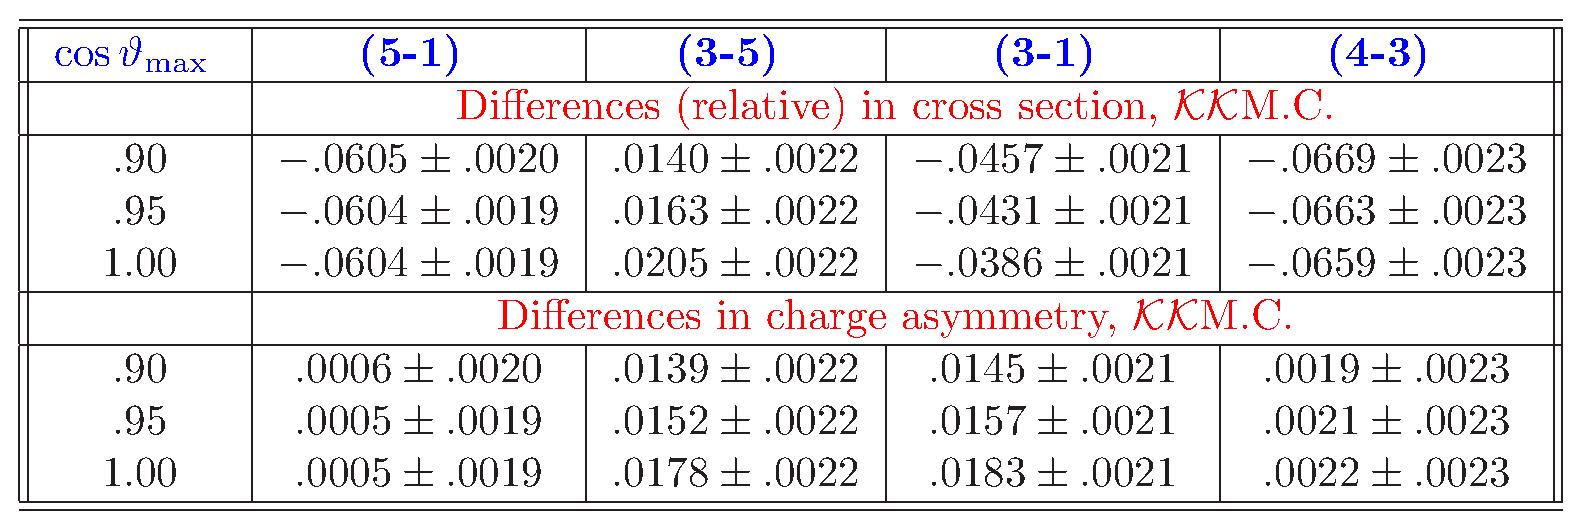
\epsfig{file=afb-int-tabEWG1.eps,width=77mm,height=25mm}
}}
\end{picture}
\end{center}

\vspace{-10mm}
\begin{center}
\setlength{\unitlength}{1mm}
\begin{picture}(80,30)
%#####\put(0,0){\framebox( 65,30){ }}
\put(-2, 00){\makebox(0,0)[lb]{
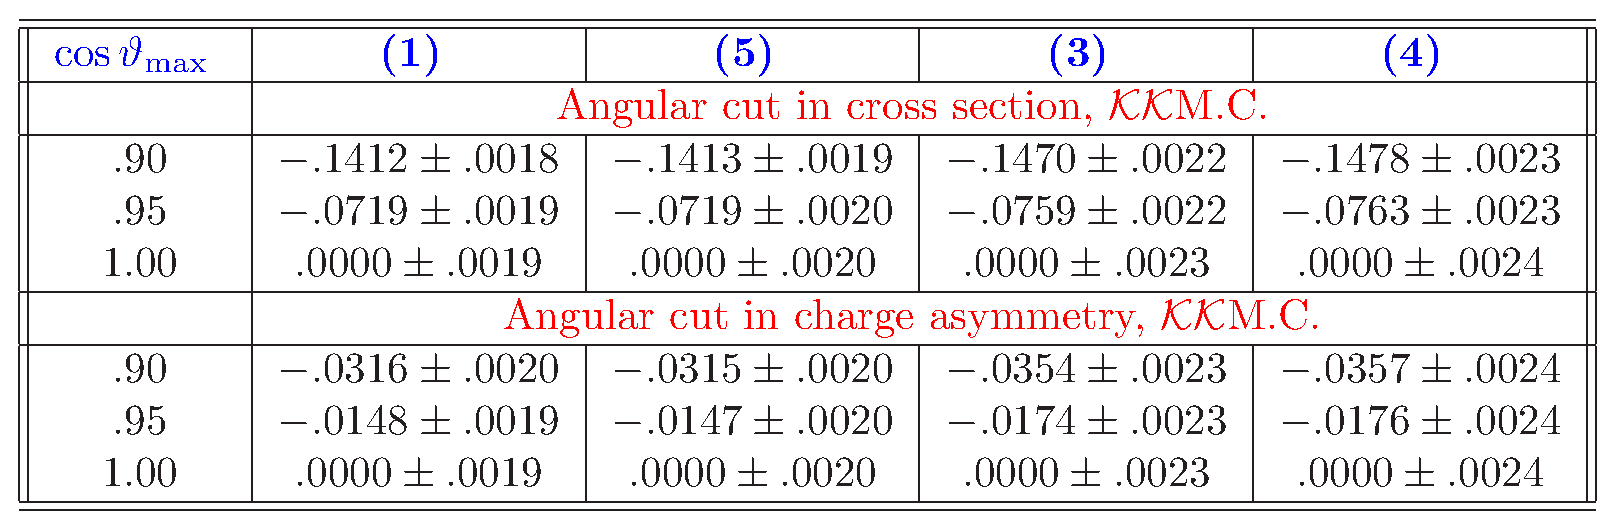
\epsfig{file=afb-int-tabEWG2.eps,width=77mm,height=25mm}
}}
\end{picture}
\end{center}

\end{PSlide}
                                                         %%%%%%%%%%%%%%%%%%%%
%%%%%%%%%%%%%%%%%%%%%%%%%%%%%%%%%%%%%%%%%%%%%%%%%%%%%%%%%%%%%%%%%%%%%%%%%%%%%


\end{document}

